\documentclass[a4paper]{article}

\usepackage{times}
\usepackage{tikz}
\usepackage[margin=0cm]{geometry}
\usepackage{graphicx}
\usepackage{anyfontsize}
\usepackage{fancyhdr}
\usepackage{indentfirst}
\usepackage{amsmath}
\usepackage[spanish]{babel}
\usepackage[utf8]{inputenc}
\usepackage{titlesec}
\usepackage{booktabs}
\usepackage{multicol}

\author{}
\date{}
\title{}

\begin{document}
\thispagestyle{empty}

\begin{tikzpicture}[remember picture, overlay]
    \pgftransformshift{\pgfpoint{0cm}{0cm}}
    \draw [line width=2pt](1cm,-1cm) -- (1cm,-27.7cm) -- (14cm, -27.7cm) -- (14cm, -1cm) -- (1cm, -1cm);
    \draw[line width=2pt] (15cm, -27.7cm) -- (19cm,-27.7cm) -- (19cm, -1cm) -- (15cm, -1cm) --  (15cm, -27.7cm);
    \node [line width=2pt] at (17cm, -3.5cm) {
\includegraphics[width=3cm]{../imagenes/utn.png}};
    \node [line width=2pt] at (7.5cm, -7.5cm) {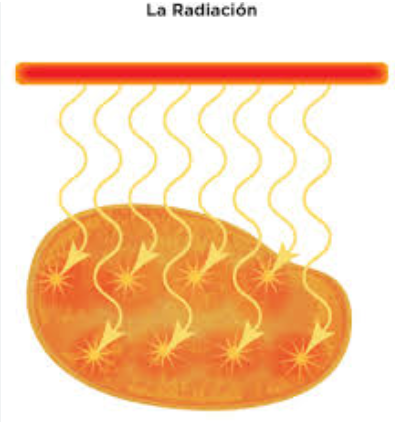
\includegraphics[width=6cm]{../imagenes/imagenCaratula.png}};
    \node at (17cm, -7cm) {\scalebox{5}{\textbf{U}}};
    \node at (17cm, -9cm) {\scalebox{5}{\textbf{T}}};
    \node at (17cm, -11cm) {\scalebox{5}{\textbf{N}}};
    \node at (17cm, -14cm) {\scalebox{5}{\textbf{F}}};
    \node at (17cm, -16cm) {\scalebox{5}{\textbf{R}}};
    \node at (17cm, -18cm) {\scalebox{5}{\textbf{C}}};
    \node at (7.5cm, -12cm) {\scalebox{2.5}{\textbf{RADIACIÓN TÉRMICA}}};

    % \node at (7cm, -24cm) {\begin{minipage}[c]{12cm}
    %     \begin{itemize}
    %         \raggedright
    %         \vspace{1.5cm}
    %         \item \fontsize{12}{12}\selectfont \textbf{Autores:} \fontsize{11}{12}\selectfont Valentino Rao (402308) - Ignacio Ismael Perea (406265) \\ Manuel Leon Parfait (406599) - Gonzalo Filsinger (400460) \\ Agustín Coronel (402010) -  Marcos Raúl Gatica (402006) \\
    %         % \fontsize{14}{14}\selectfont \textbf{Autor:} Valentino Rao. \\
    %         % \fontsize{14}{14}\selectfont \textbf{Autor:} Ignacio Ismael Perea. \\
    %         % \fontsize{14}{14}\selectfont \textbf{Autor:} Manuel Leon Parfait. \\
    %         % \fontsize{14}{14}\selectfont \textbf{Autor:} Gonzalo Filsinger. \\
    %         % \fontsize{14}{14}\selectfont \textbf{Autor:} Agustín Coronel. \\
    %         \item \fontsize{12}{12}\selectfont \textbf{Curso:} 2R1. \\
    %         \item \fontsize{12}{12}\selectfont \textbf{Asignatura:} Física Electrónica. \\
    %         \item \fontsize{12}{12}\selectfont \textbf{Institución:} Universidad Tecnológica Nacional - Facultad Regional de Córdoba. \\
    %     \end{itemize}
    % \end{minipage}};

    \node at (7.5cm, -23cm) {
        \begin{minipage}[r]{12cm}
            \begin{itemize}
                \setlength{\itemsep}{-1em}
                \item \fontsize{12}{12}\selectfont \textbf{Autores:} \vspace {1mm} \fontsize{11}{12}\selectfont 
                    \begin{itemize}
                        \setlength{\itemsep}{-1em}
                        \item \hspace{2mm} Valentino Rao - Leg. 402308 \\
                        \item \hspace{2mm} Ignacio Ismael Perea - Leg. 406265 \\
                        \item \hspace{2mm} Manuel Leon Parfait - Leg. 406599 \\ 
                        \item \hspace{2mm} Gonzalo Filsinger - Leg. 400460 \\ 
                        \item \hspace{2mm} Agustín Coronel - Leg. 402010 \\
                        \item \hspace{2mm} Marcos Raúl Gatica - Leg. 402006 \\
                        \item \hspace{2mm} Santiago Pannunzio - Leg. 402350 \\
                    \end{itemize}

                \item \fontsize{12}{12}\selectfont \textbf{Curso:} 2R1. \\
                \item \fontsize{12}{12}\selectfont \textbf{Asignatura:} Física electrónica. \\
                \item \fontsize{12}{12}\selectfont \textbf{Institución:} Universidad Tecnológica Nacional - Facultad Regional de Córdoba \\

            \end{itemize}
        \end{minipage}};


\end{tikzpicture}

\renewcommand{\normalsize}{\fontsize{12}{18}\selectfont}
\newgeometry{margin=1cm}
\fancyhf{}
\renewcommand{\headrulewidth}{0pt}
\renewcommand{\footrulewidth}{0.4pt}
\fancyfoot[R]{\textit{Rao V. - Parfait M. - Filsinger G. - Perea I. - Pannunzio S. - Coronel A. - Gatica M.} [pág. \thepage]}
% \fancyfoot[L]{\textit{Coronel A. - Leg. 402010 - 2R1 \\ Rao V. - Leg. 402308 - 2R1}}
% \fancyfoot[C]{\textit{Filsinger G. - Leg. 400460 - 2R1 \\ Gatica M. - Leg. 402006 - 2R1}}
\setlength{\footskip}{0pt}
\newpage
\thispagestyle{empty}
\text{}

\titleformat{\section} {\fontsize{12}{12}\bfseries}{\thesection.}{0.5em}{\underline}

\newpage
\newpage

\thispagestyle{empty}
\setcounter{page}{0}
\tableofcontents
\newpage
\thispagestyle{fancy}

\twocolumn
    \flushbottom
    \section{INTRODUCCIÓN}
        \subsection{La radiación térmica}
            \indent Se entiende como la radiación térmica al modo de transmitir calor de un sistema (la superficie de un cuerpo) al entorno. No requiere un medio para transmitirse, aunque es más eficaz la transmisión en el vacío. \\
            \indent Una superficie calentada a un temperatura finita interactua con el medio a menor temperatura y comienza la transmisión de calor, esto último es conocido como la radiación que emite un objeto más caliente que su entorno hasta alcanzar el equilibrio térmico. \\
            \indent La radiación que emite un sólido más caliente que su entorno se conoce como emisividad (\textbf{E}), proviene de la energía interna y la velocidad a la que la energía es emitida por la materia por su unidad de área (\textit{$\frac {W} {m^2}$}). \\
            \vspace{0mm}            

        \subsection{Radiación y las longitudes de onda}

            \indent La radiación térmica que emite un cuerpo caliente representa varias longitudes de onda. Gráficamente se puede ver que cada curva representa la variación de emisión monocromática con la long. de onda $\lambda$ \\

			\begin{figure}[h!]
				\centering
				 \includegraphics[width =5.5cm]{../imagenes/radiaciónTermVSLambda.png}
			\end{figure}

        \subsection{Experimento y objetivos}
            \indent El objetivo de este desarrollo de laboratorio es determinar la radiación térmica que emanan los siguientes materiales: \\
            \vspace{-5mm}            
            \begin{itemize}
                \setlength{\itemsep}{0pt}
                \item Plomo 
                \item Aluminio anodizado
                \item Aluminio
                \item Cobre 
                \item Chapa negra
            \end{itemize}
        
            \indent Complementario a esto, se tomará uno de los elementos seleccionados de la lista anterior para medir la radiación a cierta distancia del mismo con el fin de evaluar cómo el entorno del laboratorio influye en las mediciones de radiación. \\


     \section{REQUERIMIENTOS}
        El desarrollo del trabajo en el laboratorio requirió de los siguientes elementos:
        \subsection{El cubo de Leslie}
            \indent El cubo de Leslie permite medir y/o mostrar la energía radiada por diversos materiales en contacto con el dispositivo. 
            \newpage
            \noindent
            \indent La electrónica asociada del dispositivo empleado (con trasmisores LM-335, transductores pasivos y activos) permite obtener una sensibilidad de \textit{10mV x 1\textdegree K} \\

			\begin{figure}[h!]
				\centering
				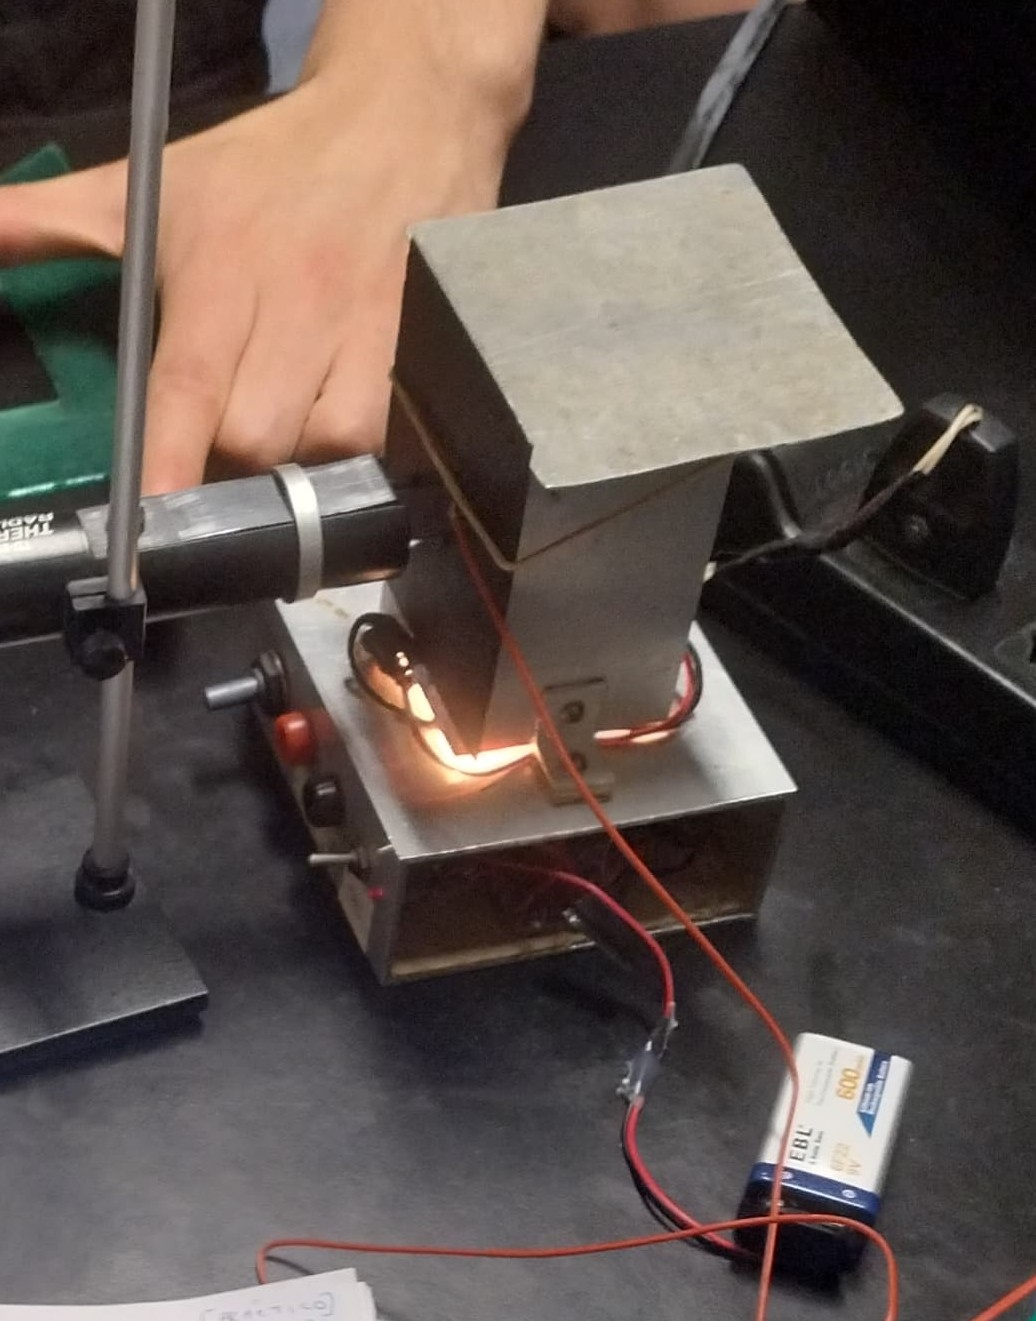
\includegraphics[width =3.5cm]{../imagenes/leslie.jpeg}
			\end{figure}

            \indent \textit{Nota: debido a un desperfecto en el instrumento, se optó por medir la temperatura de los materiales de otra forma. Naturalmente el dispositivo tiene una salida para leer los mV de la relación anteriormente mencionada.}
        \subsection{Sensor de radiación Pasco}
            \indent Este sensor lee la radiación térmica emitida por un cuerpo y devuelve un valor en mV en relación a la cantidad de mW detectados (\textit{22mV x mW}). \\
            
            \begin{figure}[h!]
            	\centering
            	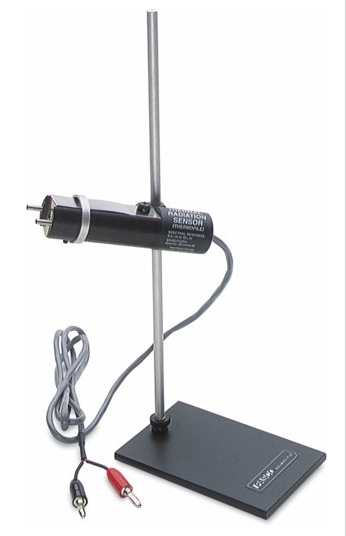
\includegraphics[width =3.5cm]{../imagenes/sensorPasco.png}
            \end{figure}
            	
        \subsection{Multímetros}
            \indent El experimento requirió de dos multímetros: uno como solución al problema del cubo de Leslie, con el cual se realizaron las mediciones de temperatura a la placa en grados Celsius usando sondas; y el restante para medir los mV del sensor Pasco.
            
            \begin{figure}[h!]
            	\centering
            	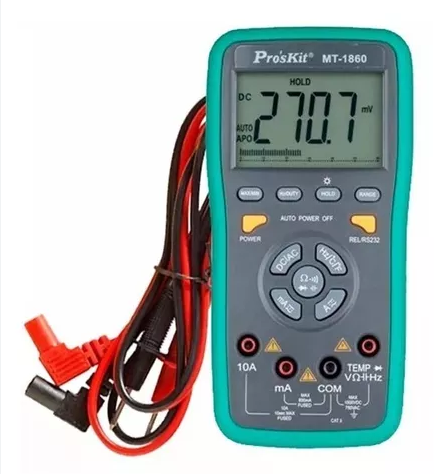
\includegraphics[width =3.5cm]{../imagenes/multimetro.png}
            \end{figure}
               
            \newpage
            \thispagestyle{fancy}
                       
    \section{PROCEDIMIENTO}
    	
        \subsection{Medición de radiación de materiales} 
	       \indent Se colocó cada placa del material en cuestión sobre la superficie del cubo de Leslie con el fin de que esta se calentase. Las siguientes tablas muestran las series de mediciones realizadas, de cada muestra, donde se registraron datos de evolución del sensor Pasco hasta una temperatura de equilibrio (donde la placa no subía más de temperatura en contacto con el cubo de Leslie): \\
	       
	       \begin{minipage}[c]{7.5cm}
	       		\centering
           		 \textit{Aluminio} 
           		\vspace{2mm}
	       \end{minipage}

            \begin{tabular}{ c  c  c  c }
                \toprule
                N \textdegree & Sensor (mV) & Rad. (mW) & Temp. (\textdegree C) \\ 
                 \midrule
                1   &   1,4  & 0,064   &   51,7 \\ 
                2   &   1,4  & 0,064   &   50,8 \\ 
                3   &   1,3  & 0,059   &   49,6 \\ 
                4   &   1,3  & 0,059   &   48,6 \\ 
                5   &   1,2  & 0,055   &   47,6 \\ 
                6   &   1,1  & 0,050   &   46,6 \\ 
                7   &   1,0  & 0,045   &   45,6 \\ 
                8   &   1,0  & 0,045   &   44,6 \\ 
                9   &   0,9  & 0,041   &   43,6 \\ 
                10  &   0,8  & 0,036   &   42,6 \\ 
                11  &   0,8  & 0,036   &   41,6 \\ 
                12  &   0,7  & 0,032   &   40,6 \\ 
                13  &   0,6  & 0,027   &   39,6 \\ 
                14  &   0,6  & 0,027   &   38,6 \\ 
                15  &   0,5  & 0,023   &   37,6 \\ 
                16  &   0,4  & 0,018   &   36,4 \\ 
                \bottomrule
            \end{tabular}

%            \textit{Cobre} 
	      	 \begin{minipage}[c]{7.5cm}
	      	 	\vspace{5mm}
				\centering
				\textit{Cobre} 
				\vspace{2mm}
			\end{minipage}
			
            \begin{tabular}{ c  c  c  c }
                \toprule
                N \textdegree & Sensor (mV) & Rad. (mW) & Temp. (\textdegree C) \\ 
                 \midrule
                1   &   1,7 & 0,077    &   51,3 \\ 
                2   &   1,6 & 0,073   &   51,5 \\ 
                3   &   1,5 & 0,068   &   50,6 \\ 
                4   &   1,4 & 0,064   &   49,6 \\ 
                5   &   1,3 & 0,059   &   48,6 \\ 
                6   &   1,2 & 0,055   &   47,1 \\ 
                7   &   1,1 & 0,050   &   45,9 \\ 
                8   &   1,0 & 0,045   &   44,7 \\ 
                9   &   0,9 & 0,041   &   43,2 \\ 
                10  &   0,8 & 0,036   &   40,7 \\ 
                11  &   0,7 & 0,032   &   40,3 \\ 
                12  &   0,6 & 0,027   &   38,8 \\ 
                \bottomrule
            \end{tabular}
            
           % \textit{Aluminio anodizado} 
	      	 \begin{minipage}[c]{7.5cm}
				\vspace{5mm}
				\centering
				\textit{Aluminio anodizado} 
				\vspace{2mm}
			\end{minipage}
			
            \begin{tabular}{ c  c  c  c }
                \toprule
                N \textdegree & Sensor (mV) & Rad. (mW) & Temp. (\textdegree C) \\
                \midrule
                1   & 2,9 & 0,132 & 50  \\ 
                2   & 2,7 & 0,123 & 49  \\ 
                3   & 2,6 & 0,118 & 48  \\ 
                4   & 2,4 & 0,109 & 47  \\ 
                5   & 2,2 & 0,100 & 46  \\ 
                6   & 2   & 0,091 & 45  \\ 
                7   & 1,9 & 0,086 & 44  \\ 
                8   & 1,8 & 0,082 & 43  \\ 
                9   & 1,6 & 0,073 & 42  \\ 
                10  & 1,5 & 0,068 & 41 \\ 
                11  & 1,3 & 0,059 & 40  \\ 
                \bottomrule
            \end{tabular}

			\newpage
			\noindent

%            \textit{Plomo} 
	      	 \begin{minipage}[c]{7.5cm}
%				\vspace{5mm}
				\centering
				\textit{Plomo} 
				\vspace{2mm}
			\end{minipage}
			
            \begin{tabular}{ c  c  c  c }
                \toprule
                N \textdegree & Sensor (mV) & Rad. (mW) & Temp. (\textdegree C) \\
                \midrule
                1   &  3,5 & 0,159 &  51  \\
                2   &  3,3 & 0,150 &  50,5 \\
                3   &  3,2 & 0,145 &  50 \\
                4   &  3   & 0,136 &  49 \\
                5   &  2,9 & 0,132 &  48 \\ 
                6   &  2,7 & 0,123 &  47 \\ 
                7   &  2,5 & 0,114 &  46 \\ 
                8   &  2,4 & 0,109 &  45 \\ 
                9   &  2,2 & 0,100 &  44 \\
                10  &  2   & 0,091 &  43 \\ 
                11  &  1,9 & 0,086 &  42 \\ 
                12  &  1,8 & 0,082 &  41 \\ 
                13  &  1,6 & 0,073 &  40 \\
                14  &  1,4 & 0,064 &  39 \\ 
                15  &  1,3 & 0,059 &  38 \\
                16  &  1,1 & 0,050 &  37 \\
                \bottomrule
            \end{tabular}
            
%            \textit{Chapa negra} 

	      	\begin{minipage}[c]{7.5cm}
				\vspace{5mm}
				\centering
				\textit{Chapa negra} 
				\vspace{2mm}
			\end{minipage}

            \begin{tabular}{ c  c  c  c }
                \toprule
                N \textdegree & Sensor (mV) & Rad. (mW) & Temp. (\textdegree C) \\
                \midrule
                1   &   3,8 & 0,173 &   51 \\
                2   &   3,6 & 0,164 &   50,4 \\
                3   &   3,5 & 0,159 &   49,5 \\
                4   &   3,3 & 0,150 &   48,8 \\
                5   &   3,1 & 0,141 &   47,5 \\
                6   &   3   & 0,136 &   46,6 \\
                7   &   2,9 & 0,132 &   45,8 \\
                8   &   2,7 & 0,123 &   45,1 \\
                9   &   2,2 & 0,100 &   42,4 \\
                10  &   2   & 0,091 &   41,5 \\
                11  &   1,9 & 0,086 &   40,4 \\
                12  &   1,7 & 0,077 &   39,4 \\
                13  &   1,5 & 0,068 &   38,5 \\
                14  &   1,4 & 0,064 &   37,9 \\
                \bottomrule
            \end{tabular}

        \subsection{Gráfico de tendencia}
            \indent En este apartado, usando los datos obtenidos de las mediciones, se realizará un gráfico de la radiación térmica en función de la temperatura de cada material.

            \begin{figure}[h!]
				\centering
				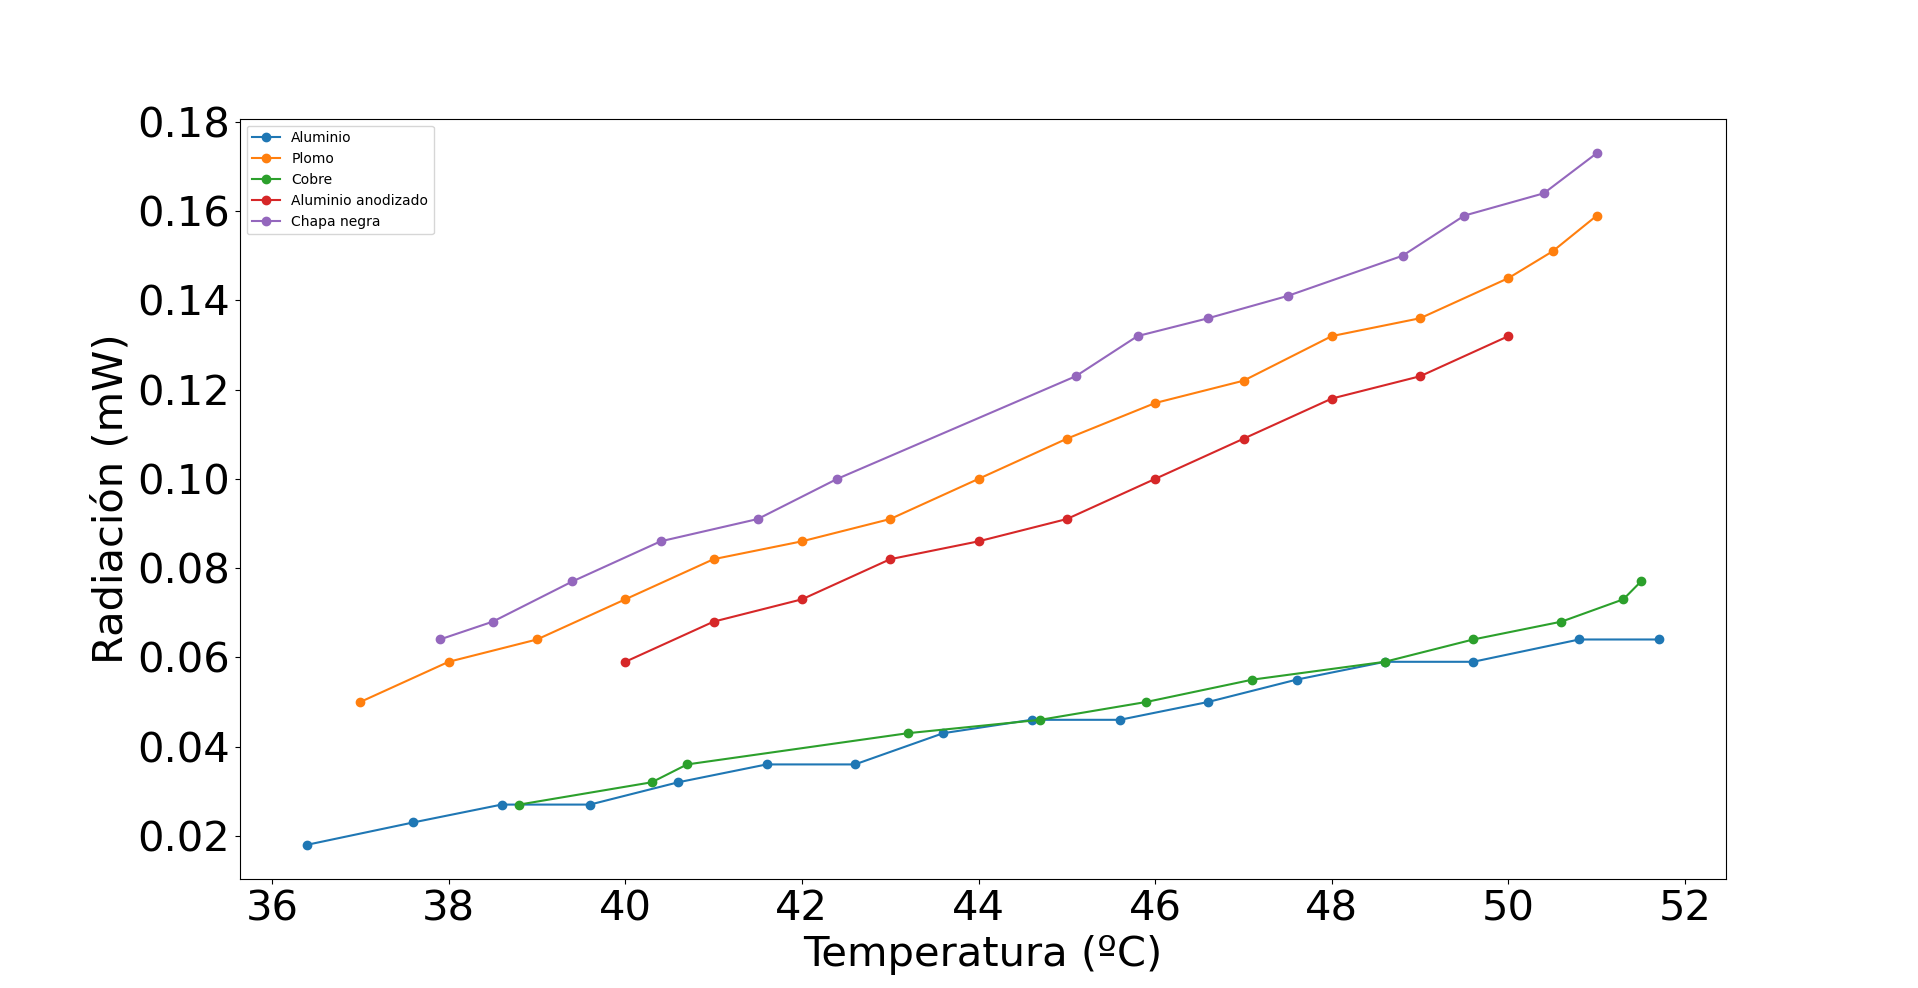
\includegraphics[width =9cm]{../imagenes/graficoRadiacionTemperatura.png}
			\end{figure}

		\newpage
		\thispagestyle{fancy}
		
		\subsection{Medición radiación a distancia}
			\indent En este apartado, se tomó al \textbf{aluminio anodizado} para medir la radiación de este a varios centímetros de la placa pegada al \textit{Cubo de Leslie} con el fin de poder estimar la radiación ambiente en el lugar de trabajo. \\
			\indent La temperatura siempre se mantuvo en ~60 \textdegree C .\\
			
		\begin{minipage}[c]{7.5cm}
			\vspace{5mm}
			\centering
			\textit{Aluminio anodizado} 
			\vspace{2mm}
		\end{minipage}
		
		\begin{tabular}{ c  c  c  c }
			\toprule
			N \textdegree & Dist. (cm) & Rad. (mW) & Sensor (mV) \\
			\midrule
			1   &   0 & 0,182 &   4   \\
			2   &   1 & 0,173 &   3,8 \\
			3   &   2 & 0,159 &   3,5 \\
			4   &   3 & 0,145 &   3,2 \\
			5   &   4 & 0,132 &   2,9 \\
			6   &   5 & 0,114 &   2,5 \\
			7   &   6 & 0,1   &   2,2 \\
			8   &   7 & 0,082 &   1,8 \\
			9   &   8 & 0,068 &   1,5 \\
			10  &   9 & 0,059 &   1,3 \\
			11  &  10 & 0,05  &   1,1 \\
			12  &  11 & 0,041 &   0,9 \\
			13  &  12 & 0,036 &   0,8 \\
			14  &  13 & 0,027 &   0,6 \\
			15  &  14 & 0,027 &   0,6 \\
			16  &  15 & 0,023 &   0,5 \\
			17  &  16 & 0,018 &   0,4 \\
			18  &  17 & 0,014 &   0,3 \\
			19  &  18 & 0,009 &   0,2 \\
			20  &  19 & 0,009 &   0,2 \\
			21  &  20 & 0,009 &   0,2 \\
			\bottomrule
		\end{tabular}
		
		\begin{itemize}
			\vspace{5mm}
			\item \textbf{Gráfico de la caída de radiación}
			\vspace{-3mm}			
		\end{itemize}
	
        \begin{figure}[h!]
			\centering
			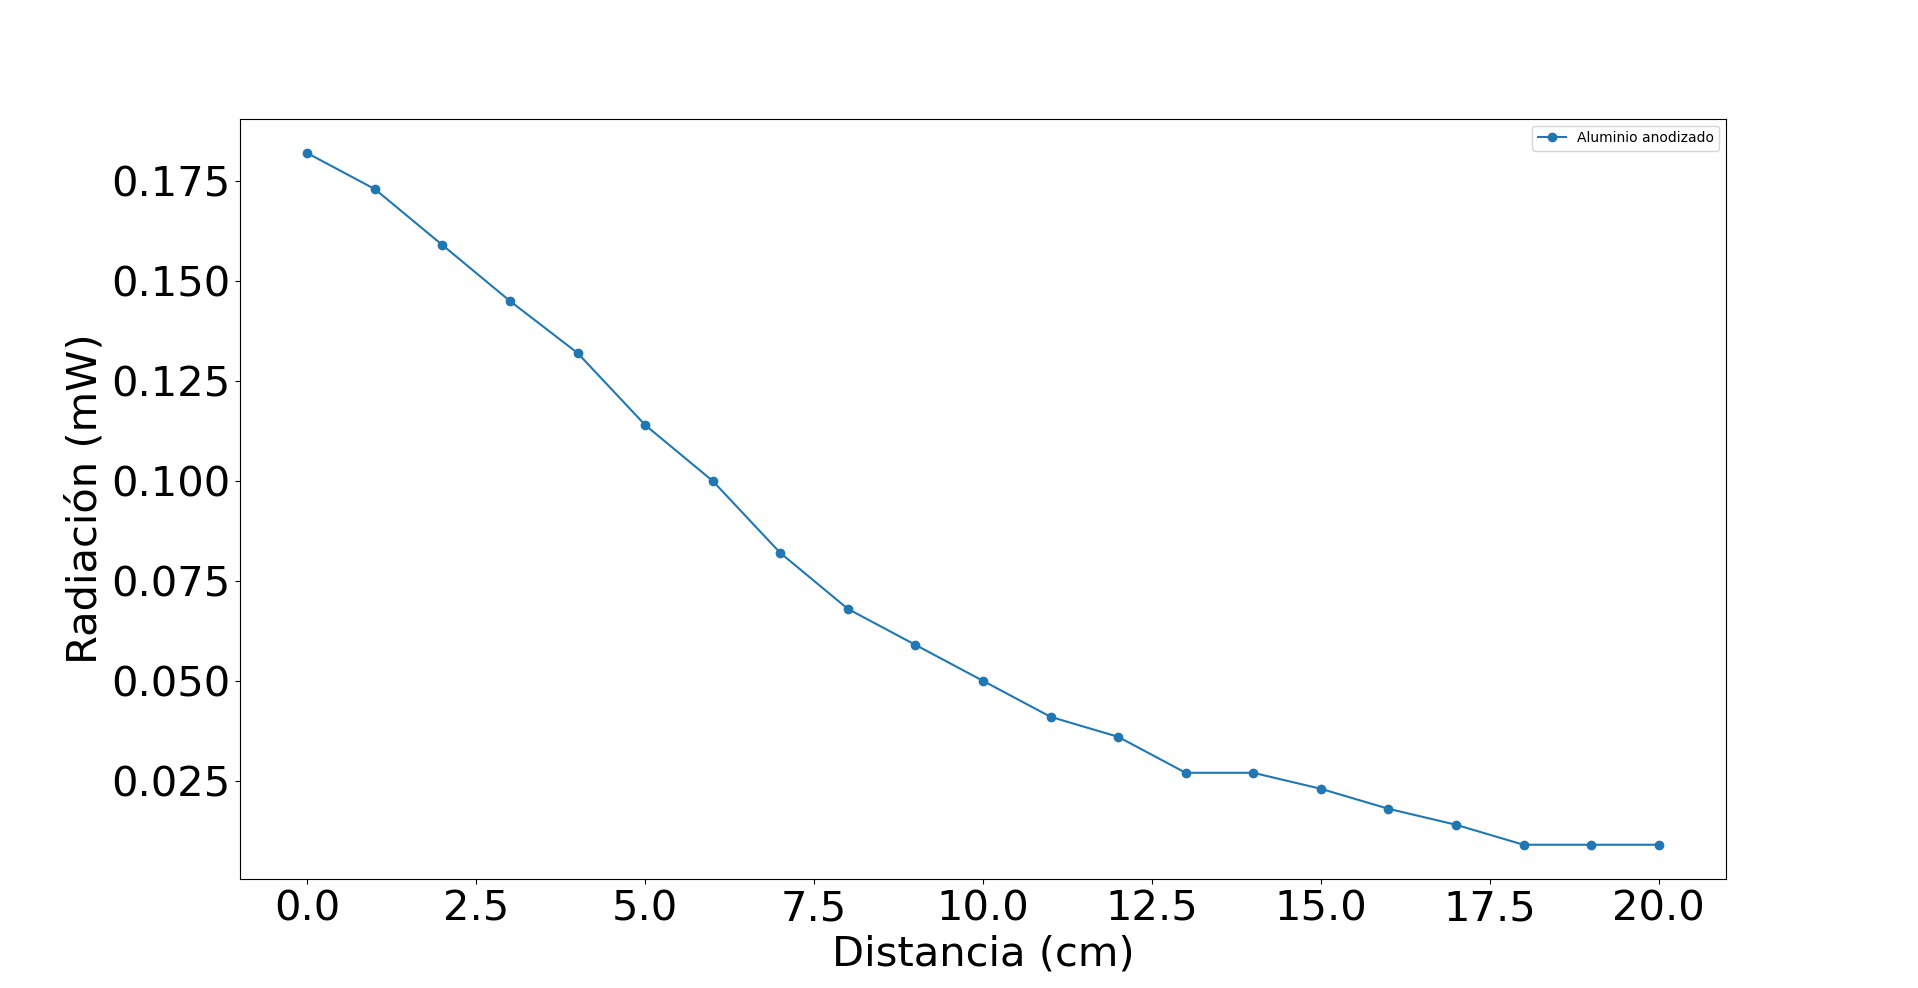
\includegraphics[width=9cm]{../imagenes/graficoRadiacionDistancia.png}
		\end{figure}
		
		\begin{itemize}
			\vspace{0mm}
			\item \textbf{Corrección de la radiación}
			\vspace{-3mm}			
		\end{itemize}
		
		\indent Para cualquier punto (preferentemente donde había más luz) en el laboratorio, el sensor Pasco midió -0,6mV (-0,02727mW) de radiación, el cual se consideró como la radiación ambiental del entorno. \\
		\indent En base a lo anterior, se puede plantear y calcular la corrección de la radiación detectada por el sensor Pasco apuntando al aluminio anodizado a cierta distancia, sabiendo que: \\
		
		\begin{center}
			$R \propto \frac{1}{d^2}$ \\
			$R_{CORREGIDA} = R_{MEDIDA} - R_{AMBIENTAL}$ \\
		\end{center}
		
		\newpage
		\noindent
		
		\begin{itemize}
			\vspace{0mm}
			\item \textbf{Tabla de correción de radiación}
			\vspace{-3mm}			
		\end{itemize}
		
		\begin{tabular}{ c  c  c  c }
			\toprule
			N \textdegree & Dist. (cm) & $Rad._{MED}$ (mW) & $Rad._{COR}$ (mW) \\
			\midrule
			1   &   0   & 0.182   & 0.209 \\
			2   &   1   & 0.173   & 0.200 \\
			3   &   2   & 0.159   & 0.186 \\
			4   &   3   & 0.145   & 0.173 \\
			5   &   4   & 0.132   & 0.159 \\
			6   &   5   & 0.114   & 0.141 \\
			7   &   6   & 0.1  	  & 0.127 \\
			8   &   7   & 0.082   & 0.109 \\
			9   &   8   & 0.068   & 0.095 \\
			10  &   9   & 0.059   & 0.086 \\
			11  &   10  & 0.05    & 0.077 \\
			12  &   11  & 0.041   & 0.068 \\
			13  &   12  & 0.036   & 0.064 \\
			14  &   13  & 0.027   & 0.055 \\
			15  &   14  & 0.027   & 0.055 \\
			16  &   15  & 0.023   & 0.050 \\
			17  &   16  & 0.018   & 0.045 \\
			18  &   17  & 0.014   & 0.041 \\
			19  &   18  & 0.009   & 0.036 \\
			20  &   19  & 0.009   & 0.036 \\
			21  &   20  & 0.009   & 0.036 \\
			\bottomrule
		\end{tabular}

	\section{CONCLUSIONES}
		\indent El trabajo de laboratorio permitió concluir en que la transmisión de la emisión de la radiación se basa en ondas electromagnéticas infrarrojas capaz de ser medidas por una electrónica concreta como el sensor Pasco. \\
		\indent Además, se puede concluir que la emisión de radiación de un cuerpo depende de la cantidad de calor que este tenga. Experimentos como estos pueden servir para determinar la capacidad disipativa de un material con el fin de hacer refrigeraciones mejores (por tener mayor capacidad de extraer el calor de un sistema haciendo trabajo, para llevarlo al entorno). \\
		\indent Con respecto a la radiación ambiental, se puede apreciar que tiene un impacto en las mediciones a medida que la distancia a un objeto emisor radioactivo aumenta. Un entorno más "limpio" de radiación puede llevar a conclusiones como: \\
		
		\begin{center}
			$R_{MEDIDA} \approx R_{MEDIDA + DISTANCIA}$
		\end{center}
		
    \indent Sin embargo, notése que que el plomo está por debajo del aluminio, y entre estos materiales es el que mejor capacidad disipativa tiene. Por lo que da a entender que lo primero es falso.\\
    \indent Hay que tener en cuenta que el ensayo que se realizó no tuvo en cuenta algunos puntos: los instrumentos no son muy rigurosos en términos de precisión, y que el sensor Pasco tiende a saturar bien después de una hora de lectura. 

\end{document}


